\documentclass[crop,tikz,convert]{standalone}
\usetikzlibrary{shapes,matrix,positioning,chains,arrows,shadows,decorations.pathmorphing,fit,backgrounds}
\begin{document}
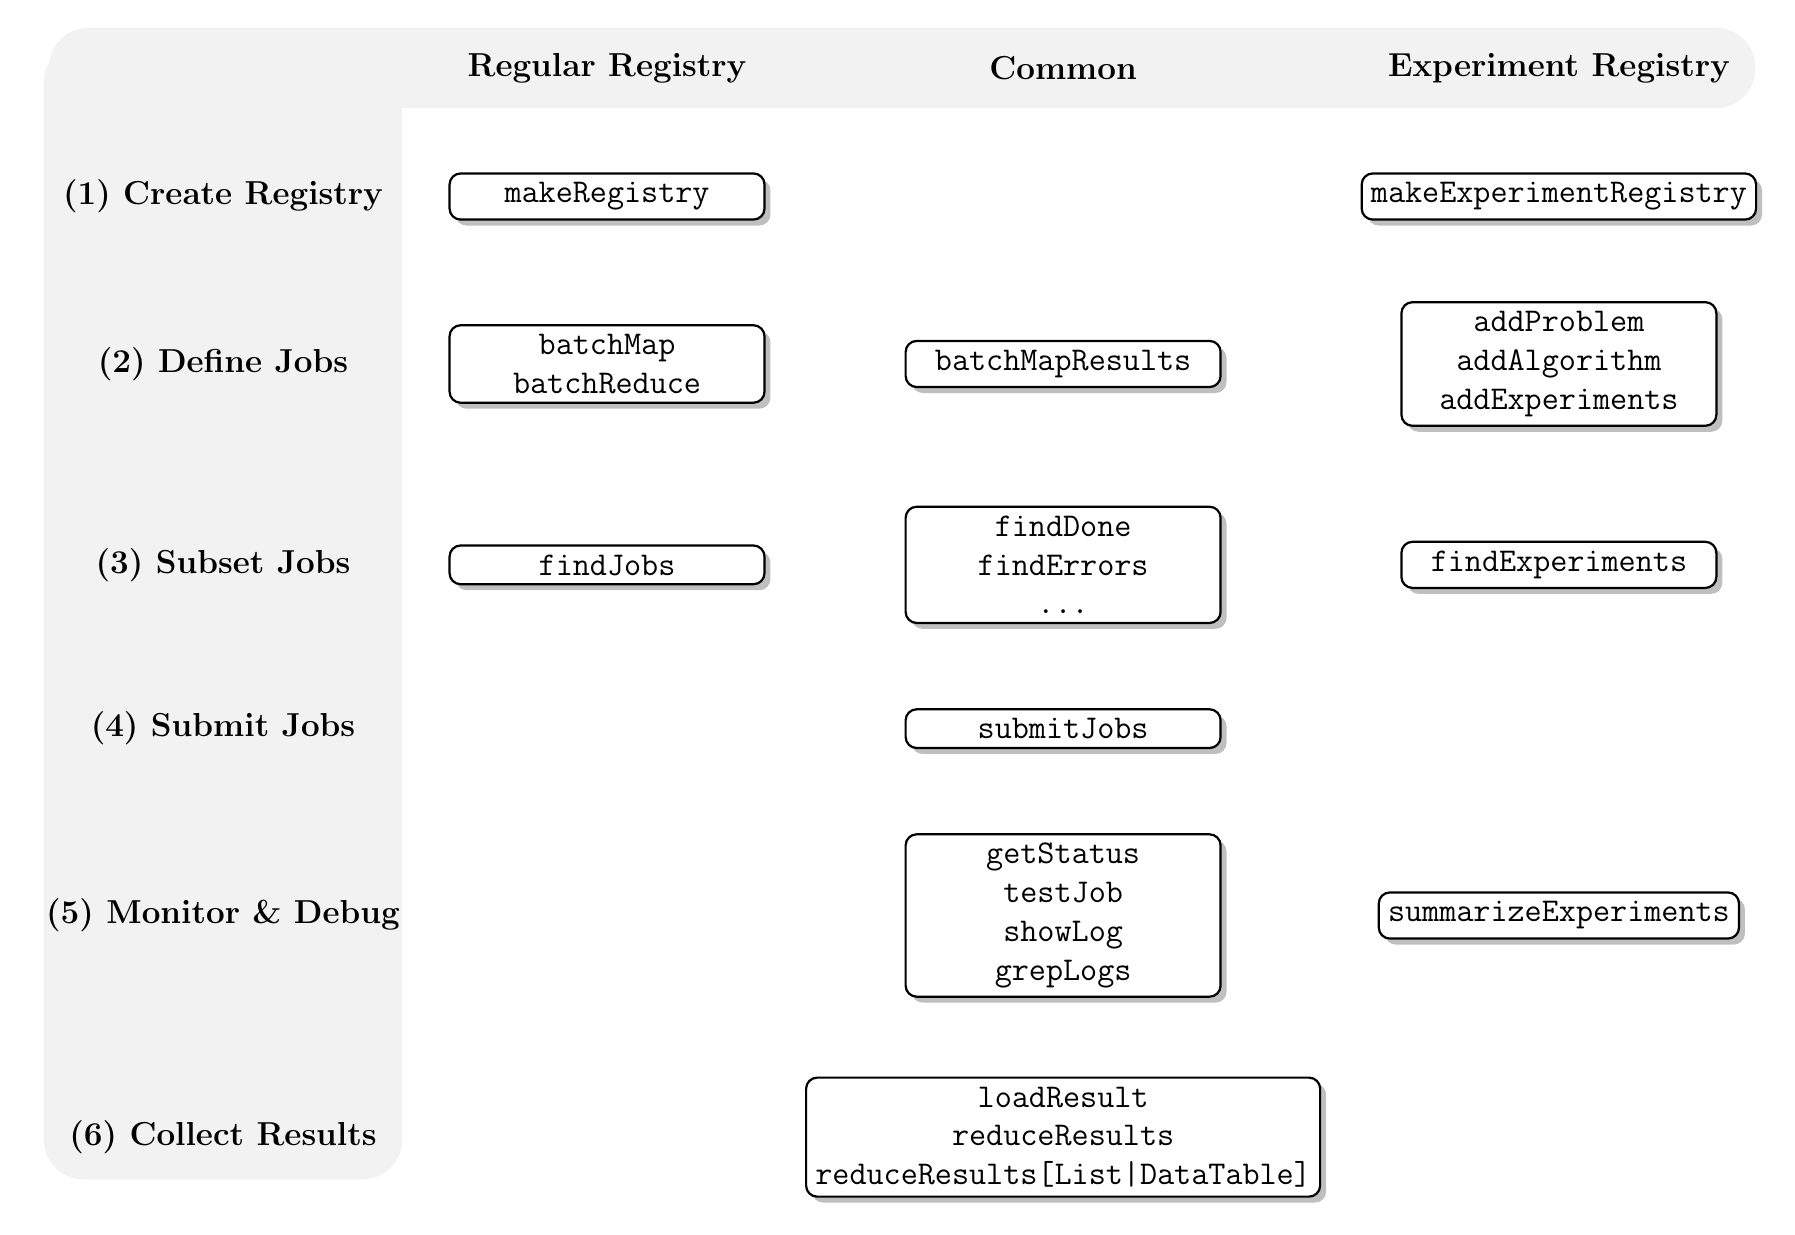
\begin{tikzpicture}[auto]
  \tikzstyle{box} = [rectangle, drop shadow, draw=black, fill=white, thick, minimum width=4cm, rounded corners, align=center,font=\ttfamily\large]
  \tikzstyle{chead} = [font=\large\bfseries]
  \tikzstyle{rhead} = [chead,align=left, minimum width=4cm]
  \tikzstyle{bg} = [rectangle, fill=gray!10, inner sep=0.2cm, rounded corners=5mm]
  \tikzstyle{hl} = [rectangle, draw=red, inner sep=0.2cm, rounded corners=5mm]

  \matrix [row sep=10mm, column sep=5mm] (mat) {
    \node (chead0) [minimum width=4cm] {}; \pgfmatrixnextcell
    \node (chead1) [chead] {Regular Registry}; \pgfmatrixnextcell
    \node (chead2) [chead] {Common}; \pgfmatrixnextcell
    \node (chead3) [chead] {Experiment Registry}; \\

    \node (registry0) [rhead] {(1) Create Registry}; \pgfmatrixnextcell
    \node (registry1) [box] {makeRegistry}; \pgfmatrixnextcell
    \node (registry2) {}; \pgfmatrixnextcell
    \node (registry3) [box] {makeExperimentRegistry}; \\

    \node (define0) [rhead] {(2) Define Jobs}; \pgfmatrixnextcell
    \node (define1) [box] {batchMap \\ batchReduce}; \pgfmatrixnextcell
    \node (define2) [box] {batchMapResults}; \pgfmatrixnextcell
    \node (define3) [box] {addProblem \\ addAlgorithm \\ addExperiments}; \\

    \node (subsetting0) [rhead] {(3) Subset Jobs}; \pgfmatrixnextcell
    \node (subsetting1) [box] {findJobs}; \pgfmatrixnextcell
    \node (subsetting2) [box] {findDone\\ findErrors \\\ldots}; \pgfmatrixnextcell
    \node (subsetting3) [box] {findExperiments}; \\

    \node (submit0) [rhead] {(4) Submit Jobs}; \pgfmatrixnextcell
    \node (submit1) {}; \pgfmatrixnextcell
    \node (submit2) [box] {submitJobs}; \pgfmatrixnextcell
    \node (submit3) {}; \\

    \node (status0) [rhead] {(5) Monitor \& Debug}; \pgfmatrixnextcell
    \node (status1) {}; \pgfmatrixnextcell
    \node (status2) [box] {getStatus \\ testJob \\ showLog \\ grepLogs}; \pgfmatrixnextcell
    \node (status3) [box] {summarizeExperiments}; \\

    \node (collect0) [rhead] {(6) Collect Results}; \pgfmatrixnextcell
    \node (collect1) {}; \pgfmatrixnextcell
    \node (collect2) [box] {loadResult \\ reduceResults \\ reduceResults[List|DataTable]}; \pgfmatrixnextcell
    \node (collect3) {}; \\
  };
  \begin{pgfonlayer}{background}
    \node [bg, fit=(chead0) (collect0)] {};
    \node [bg, fit=(chead0) (chead3)] {};
  \end{pgfonlayer}
\end{tikzpicture}
\end{document}
